\documentclass[journal,twoside,web]{ieeecolor}
\usepackage{generic}
\usepackage{cite}
\usepackage{amsmath,amssymb,amsfonts}
\usepackage{algorithmic}
\usepackage{graphicx}
\usepackage{textcomp}
\def\BibTeX{{\rm B\kern-.05em{\sc i\kern-.025em b}\kern-.08em
    T\kern-.1667em\lower.7ex\hbox{E}\kern-.125emX}}
\markboth{\journalname, VOL. XX, NO. XX, XXXX 2017}
{Author \MakeLowercase{\textit{et al.}}: Preparation of Papers for IEEE TRANSACTIONS and JOURNALS (February 2017)}
\begin{document}
\title{Santander Customer Transaction Prediction (March 2019)}\\

\author{Adam Kulas, Ammar Ahmed, and Richard Ozara\\
\institute University of Waterloo,ON N2L 3G1, Canada\\akulas@uwaterloo.ca\\
a272ahme@uwaterloo.ca \\\centerline{roozara@uwaterloo.ca}}

\maketitle



\begin{abstract}
This paper lays down the process and detailed approach attempted to solve a binary classification problem presented by Santander bank. Different machine learning algorithms were explored and implemented and comparison was made among them. All the programming was done in python using different libraries and packages. The paper focuses more on the application oriented domain (high level implementation and evaluation of the chosen models) and does not cover in depth explanation of those implemented algorithms. 

\end{abstract}

\begin{IEEEkeywords}
Binary classification, Boosting, Ensembling, Machine learning, Naive Bayes, lgbm, logistic regression, XGBoost

\end{IEEEkeywords}

\section{Introduction}
\label{sec:introduction}
\IEEEPARstart{T}{he} purpose of this project is to solve a problem presented by the company Santander. Santander is a bank that is originating in Spain. Since 2013 they have been serving customers in northeastern North America. Santander mentions in the competition description that their most common problems are binary classification problems. The main goal for the competition is to predict which customers will make a specific transaction in the future, irrespective of money transacted. The problem presented by this challenge is a binary classification problem. The challenge is hosted on Kaggle.com where competitors submit their predicted results online and are evaluated on area under the (ROC) curve between the predicted probability and the observed target. The approach followed in this paper started with data preprocessing and then to data exploration and visualization. After that, a simple random forest model was created to set a baseline performance bench-mark and to help with extracting important features as part of the exploratory data analysis (EDA). Then, implemented supervised machine learning classffication algorithms such as naive bayes and logistic regression that were more specifically tailored to the dataset and problem space. Lastly, a more advanced models were tested such XGBoost and LGBM which required a lot of exploring and tuning their hyperparamters. Also, techniques such ensembling models were tested and all results were compared and evaluated. Throughout the process of testing those models, cross-validation CV was performed and cross-referenced with kaggle leader board scores.

\subsection{Abbreviations and Acronyms}
CV score = Cross Validation score \\

\section{Description of the data}
The dataset used in this project is provided by Santander and can be downloaded from kaggle.com. There are two main files: train.csv which contains the training set and the test.csv which contains the test set. The size of the train.csv is 200k x 201 (40,200,000 data points) and for the tain.csv is 200k x 202 (40,000,000 data points). The train.csv has the attributes: binary target column, string ID\_code column, and the numeric feature variables (var0 till var 199) while the test.csv contains the string ID\_code and the numeric feature variables, so the task is to predict the value of target column in the test set. The datasets are fully anonymized. Test labels (target) is private - predicted results must be submitted online and submissions are evaluated on area under the ROC curve between the predicted probability and the observed target. Lastly, there are three submissions resets every 24hrs.

\section{Survey review on the dataset}


\section{Challenges in the dataset}
Fully anonymized dataset.\\
Imbalance dataset.




\begin{center}
 \begin{tabular}{||c c c c||} 
 \hline
 Target Variable & Percentage \\ [0.5ex] 
 \hline\hline
 0 & 89.5  \\ 
 \hline
 1 & 10.5 \\[1ex]
 \hline
\end{tabular}
\end{center}







\section{Preprocessing}
For the data preprocessing, missing values were checked first and there was no missing values found. However, the proportion of the data imbalance found was significant with 89.95\% (179,902 samples) of the target label in the train.csv were classified as 0 as compared to 10.05\% of the data labeled as 1 (20,098 samples). This means that there are two options that should be considered, either up-sample minority class or down-sample majority class. Most cases, down sampling is the optimal option, however, there are some cases were upsampling gives an optimal results over the downsampling depending on the type of the dataset. Another options (besides up and downsampling) are either changing the perfomance metrics or penalize algorithms (Cost-Sensitive Training). As far as this project is concerned, both upsampling and downsampling were performed to compare the results. Lastly, the data was normalized using z-score normalization. Even though not all models need a normalized data (such as XGBoost and LGBM), normalizing for all models helps in making a fair evaluation and comparison of the performances of those models. 


\section{exploratory data analysis (EDA)}
EDA refers to the critical process of performing initial investigations on data so as to discover patterns,to spot anomalies,to test hypothesis and to check assumptions with the help of summary statistics and graphical representations [reference: https://towardsdatascience.com/exploratory-data-analysis-8fc1cb20fd15].
The first part of the EDA was checking for linear correlation between the features. Those identified relationship should be removed during feature selection as they effect some of the models such linear regression. However, for this specific dataset it was foound that all 200 features had a correlation coefficient value between -0.1 and 0.1, which indicates that there is no linear relationship between those 200 features. The heatmap (figure~\ref{fig:fig1}) below shows the results of correlation in which it can be observed that it is almost zero. 
\begin{figure}[h!]
  \centering
  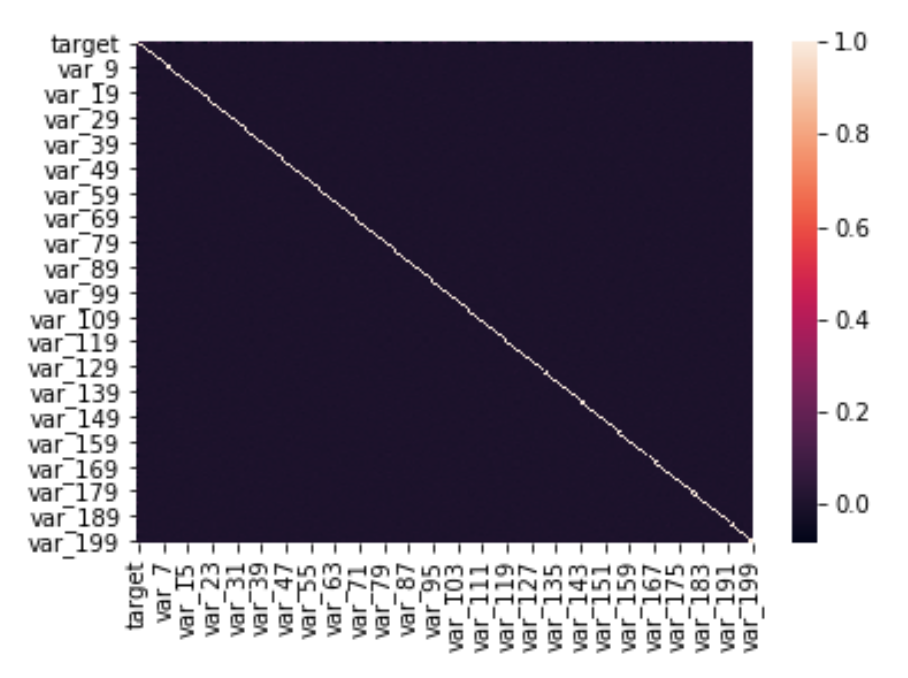
\includegraphics[width=3.8in]{project/code/heatmap.png}
  \caption{Heatmap for correlation}
  \label{fig:fig1}
\end{figure}

Since there are 200 features, it is a bit difficult to plot histograms and box plots for all those features, however, to make the task easier, PCA was first used reduce the dimensionality. When running the PCA (figure~\ref{fig:fig2} below), it can be observed that almost all of the 200 features are required to explain 95\% of the variance. Examining the PCA plot, it is possible that the provider of the dataset already have done some preprocessing techniques, PCA possibly. 
\begin{figure}[h!]
  \centering
  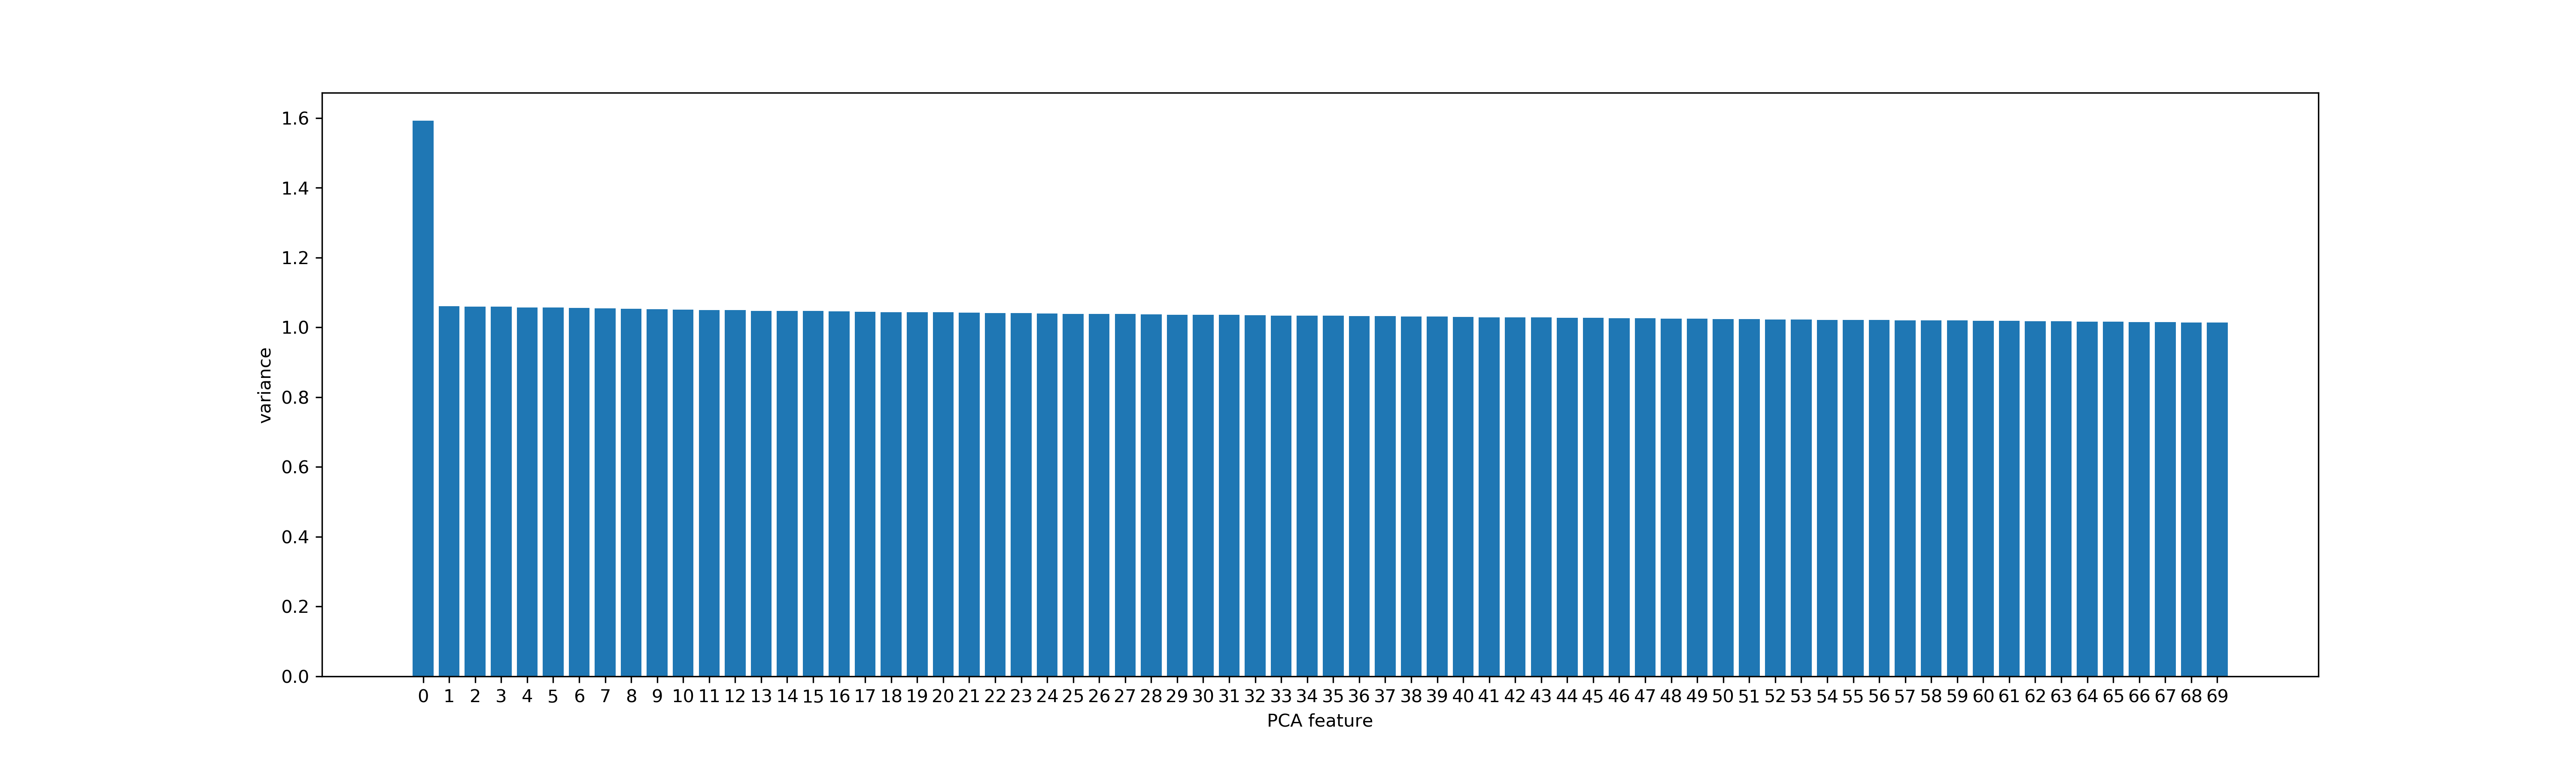
\includegraphics[width=4.1in]{project/code/1-pcafeatures.png}
  \caption{PCA}
  \label{fig:fig2}
\end{figure}
Next thing was to build a simple random forest model to extract important features and possibly providing more insights to the dataset. 


\section{Project Goal}




\section{Used Methods in the Project}


\subsection{Naive Bayes}



\subsection{Logistic Regression}


\subsection{XGBOOST}


\subsection{LGBM}









\subsection{Checking Your Figures: The IEEE Graphics Analyzer}
located at
\underline{http://graphicsqc.ieee.org/}, allows authors to 




\subsection{Color Processing/Printing in IEEE Journals}
IEEE Xplore\textregistered\ at no charge, 

\section{Conclusion}
A conclusion section is not required. Although a conclusion may review the 
main points of the paper, do not replicate the abstract as the conclusion. A 
conclusion might elaborate on the importance of the work or suggest 
applications and extensions. 

\appendices

Appendixes, if needed, appear before the acknowledgment.

\section*{Acknowledgment}



\section*{References and Footnotes}

\subsection{References}






\begin{thebibliography}{00}

\bibitem{b1} G. O. Young, ``Synthetic structure of industrial plastics,'' in \emph{Plastics,} 2\textsuperscript{nd} ed., vol. 3, J. Peters, Ed. New York, NY, USA: McGraw-Hill, 1964, pp. 15--64.

\bibitem{b2} W.-K. Chen, \emph{Linear Networks and Systems.} Belmont, CA, USA: Wadsworth, 1993, pp. 123--135.

\bibitem{b3} J. U. Duncombe, ``Infrared navigation---Part I: An assessment of feasibility,'' \emph{IEEE Trans. Electron Devices}, vol. ED-11, no. 1, pp. 34--39, Jan. 1959, 10.1109/TED.2016.2628402.

\bibitem{b4} E. P. Wigner, ``Theory of traveling-wave optical laser,'' \emph{Phys. Rev}., vol. 134, pp. A635--A646, Dec. 1965.

\bibitem{b5} E. H. Miller, ``A note on reflector arrays,'' \emph{IEEE Trans. Antennas Propagat}., to be published.

\bibitem{b6} E. E. Reber, R. L. Michell, and C. J. Carter, ``Oxygen absorption in the earth's atmosphere,'' Aerospace Corp., Los Angeles, CA, USA, Tech. Rep. TR-0200 (4230-46)-3, Nov. 1988.

\bibitem{b7} J. H. Davis and J. R. Cogdell, ``Calibration program for the 16-foot antenna,'' Elect. Eng. Res. Lab., Univ. Texas, Austin, TX, USA, Tech. Memo. NGL-006-69-3, Nov. 15, 1987.

\bibitem{b8} \emph{Transmission Systems for Communications}, 3\textsuperscript{rd} ed., Western Electric Co., Winston-Salem, NC, USA, 1985, pp. 44--60.

\bibitem{b9} \emph{Motorola Semiconductor Data Manual}, Motorola Semiconductor Products Inc., Phoenix, AZ, USA, 1989.

\bibitem{b10} G. O. Young, ``Synthetic structure of industrial
plastics,'' in Plastics, vol. 3, Polymers of Hexadromicon, J. Peters,
Ed., 2\textsuperscript{nd} ed. New York, NY, USA: McGraw-Hill, 1964, pp. 15-64.
[Online]. Available:
\underline{http://www.bookref.com}.



\end{thebibliography}






\end{document}
